% =====================================================================
%  From Idea to Sheet Music: Two Halves of One Music-AI System
%  Joint lab presentation — Harry Ilanyan + Antoine — Bayen Lab
%  Built to follow LAB_PRESENTATION_SCRIPT.md slide-for-slide.
%  Compile:  tectonic LAB_PRESENTATION.tex
%  Speaker script is embedded as \note{} (hidden by default).
%  To print notes:  uncomment \setbeameroption{show notes} below.
% =====================================================================
\documentclass[aspectratio=169,11pt]{beamer}

\usepackage[T1]{fontenc}
\usepackage{helvet}
\renewcommand{\familydefault}{\sfdefault}
\usepackage{booktabs}
\usepackage{tikz}
\usetikzlibrary{arrows.meta,positioning,calc,shapes.geometric,fit,backgrounds,shapes.misc}

% ---------- colour palette ----------
\definecolor{labblue}{RGB}{24,72,110}     % primary (deep teal-navy)
\definecolor{labaccent}{RGB}{198,92,28}   % accent (rust / amber)
\definecolor{labgreen}{RGB}{36,120,90}    % success
\definecolor{labgray}{RGB}{95,99,104}
\definecolor{boxblue}{RGB}{225,236,244}
\definecolor{boxgray}{RGB}{236,237,239}
\definecolor{boxamber}{RGB}{250,235,220}
\definecolor{boxgreen}{RGB}{224,239,232}
\definecolor{boxred}{RGB}{248,228,224}

% ---------- theme ----------
\usetheme{default}
\setbeamertemplate{navigation symbols}{}
\setbeamercolor{structure}{fg=labblue}
\setbeamercolor{title}{fg=labblue}
\setbeamercolor{frametitle}{fg=labblue}
\setbeamercolor{itemize item}{fg=labaccent}
\setbeamercolor{itemize subitem}{fg=labgray}
\setbeamerfont{frametitle}{series=\bfseries,size=\large}
\setbeamerfont{title}{series=\bfseries}
\setbeamertemplate{itemize item}{\textbullet}
\setbeamertemplate{itemize subitem}{--}

\setbeamertemplate{frametitle}{%
  \vspace{0.5em}\hspace{0.2em}{\usebeamerfont{frametitle}\usebeamercolor[fg]{frametitle}\insertframetitle}\par
  \vspace{-0.35em}{\color{labaccent}\rule{\textwidth}{1.2pt}}\par}

\setbeamertemplate{footline}{%
  \hbox{\begin{beamercolorbox}[wd=\paperwidth,ht=2.6ex,dp=1.1ex,leftskip=1.2em,rightskip=1.2em]{}%
  {\scriptsize\color{labgray} From Idea to Sheet Music \hfill Harry + Antoine \,$\cdot$\, Bayen Lab \hfill \insertframenumber/\inserttotalframenumber}%
  \end{beamercolorbox}}}

% section divider frames
\AtBeginSection[]{%
  \begin{frame}[plain]
    \centering
    \vfill
    {\color{labgray}\footnotesize ACT \insertsectionnumber}\par\vspace{0.4em}
    {\color{labblue}\Huge\bfseries \insertsectionhead}\par
    \vspace{0.6em}{\color{labaccent}\rule{0.35\textwidth}{1.4pt}}
    \vfill
  \end{frame}}

% ---------- reusable tikz styles ----------
\tikzset{
  pbox/.style={rounded corners=3pt, draw=labblue, fill=boxblue, line width=0.8pt,
               text width=2.6cm, align=center, minimum height=1.1cm, font=\small},
  dbox/.style={rounded corners=3pt, draw=labgray, fill=boxgray, line width=0.8pt,
               text width=2.4cm, align=center, minimum height=1.0cm, font=\small},
  abox/.style={rounded corners=3pt, draw=labaccent, fill=boxamber, line width=1.0pt,
               text width=2.8cm, align=center, minimum height=1.1cm, font=\small},
  shared/.style={rounded corners=4pt, draw=labaccent, fill=boxamber, line width=1.4pt,
               text width=3.6cm, align=center, minimum height=1.4cm, font=\small\bfseries},
  flow/.style={-{Stealth[length=3mm]}, line width=1.1pt, draw=labblue},
  flowa/.style={-{Stealth[length=3mm]}, line width=1.3pt, draw=labaccent},
}

% mini staff-with-notes glyph: \miniscore{<x>}{<y>}{<scale>}
\newcommand{\miniscore}[3]{%
  \begin{scope}[shift={(#1,#2)}, scale=#3]
    \foreach \l in {0,0.18,0.36,0.54,0.72}{\draw[labgray, line width=0.5pt] (0,\l) -- (2.4,\l);}
    \foreach \nx/\ny in {0.45/0.18, 0.95/0.45, 1.4/0.36, 1.9/0.63}{
      \filldraw[labblue] (\nx,\ny) ellipse (0.12 and 0.085);
      \draw[labblue, line width=0.7pt] (\nx+0.11,\ny) -- (\nx+0.11,\ny+0.5);}
  \end{scope}}

% small "optional tech" tag
\newcommand{\techtag}{{\color{labgreen}\footnotesize\textbf{[Tech, optional $\sim$10s]}}}

% ---------- title metadata ----------
\title{\textbf{From Idea to Sheet Music}}
\subtitle{Two halves of one music-AI system}
\author{Harry Ilanyan \quad\textbullet\quad Antoine}
\institute{Bayen Lab}
\date{}

% \setbeameroption{show notes}   % <-- uncomment to print speaker notes

\begin{document}

% =====================================================================
% ACT 0 — THE VISION
% =====================================================================

% ---- Slide 0.1 — Title ----
\begin{frame}[plain]
  \vfill
  \centering
  {\color{labblue}\Huge\bfseries From Idea to Sheet Music}\par
  \vspace{0.3em}{\color{labgray}\large Two halves of one music-AI system}\par
  \vspace{0.5em}{\color{labaccent}\rule{0.4\textwidth}{1.4pt}}\par
  \vspace{1.0em}
  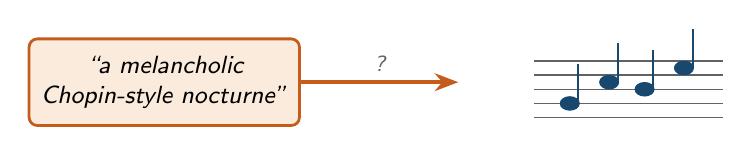
\begin{tikzpicture}
    \node[abox, text width=3.2cm] (txt) {\textit{``a melancholic\\ Chopin-style nocturne''}};
    \node[right=2.2cm of txt] (sc) {};
    \draw[flowa] (txt.east) -- node[above,font=\footnotesize\itshape,color=labgray]{?} ($(sc.west)+(-0.2,0)$);
    \miniscore{4.7}{-0.45}{1.0}
  \end{tikzpicture}\par
  \vspace{1.0em}
  {\color{labgray}\normalsize Harry Ilanyan \quad\textbullet\quad Antoine \quad\textbullet\quad Bayen Lab}
  \vfill
  \note{(Harry) ``Hi everyone. Antoine and I have been working on what look like two separate projects --- he generates music, I turn performances into sheet music. Today we want to show you they're actually one project, and that they meet in a surprising place. Let's start with the dream.''}
\end{frame}

% ---- Slide 0.2 — The Dream ----
\begin{frame}{The dream}
  \vfill
  \centering
  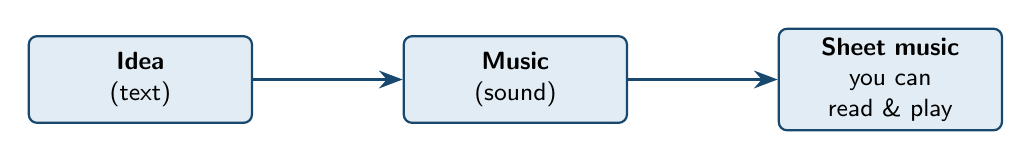
\begin{tikzpicture}[node distance=1.9cm]
    \node[pbox] (idea) {\textbf{Idea}\\ (text)};
    \node[pbox, right=of idea] (music) {\textbf{Music}\\ (sound)};
    \node[pbox, right=of music] (score) {\textbf{Sheet music}\\ you can read \& play};
    \draw[flow] (idea) -- (music);
    \draw[flow] (music) -- (score);
  \end{tikzpicture}
  \vfill
  \begin{block}{}
    \centering Type \textit{``a melancholic Chopin-style nocturne''} $\to$ get \textbf{audio} \emph{and} a clean, playable \textbf{score}.
  \end{block}
  \vfill
  \note{(Antoine) ``The north star --- Prof. Bayen's direction --- is this: a musician, a student, anyone, types an idea in plain language and gets back real, performable sheet music. To get there you need two capabilities. One: a model that creates music. Two: a model that can take sound --- a performance, a recording, or generated audio --- and write it down as a correct score. I build the first half. Harry builds the second. And the punchline of today is that the hard part of both is the same part.''}
\end{frame}

% ---- Slide 0.3 — The Map ----
\begin{frame}{The lab on one slide}
  \centering
  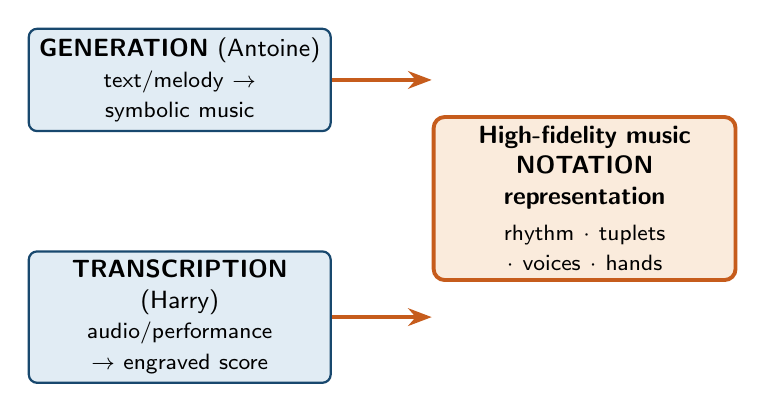
\begin{tikzpicture}[node distance=1.0cm]
    \node[pbox, text width=3.6cm] (gen) {\textbf{GENERATION} (Antoine)\\ \footnotesize text/melody $\to$ symbolic music};
    \node[pbox, text width=3.6cm, below=1.5cm of gen] (trn) {\textbf{TRANSCRIPTION} (Harry)\\ \footnotesize audio/performance $\to$ engraved score};
    \node[shared, right=3.2cm of $(gen)!0.5!(trn)$] (rep) {High-fidelity music\\ NOTATION representation\\[2pt] \footnotesize\mdseries rhythm $\cdot$ tuplets $\cdot$ voices $\cdot$ hands};
    \draw[flowa] (gen.east) -- (rep.west|-gen.east);
    \draw[flowa] (trn.east) -- (rep.west|-trn.east);
  \end{tikzpicture}
  \vspace{0.6em}
  \begin{center}\color{labgray}\itshape Different inputs, same core problem.\end{center}
  \note{(Harry) ``Here's the map. Antoine's half goes from an idea to music. My half goes from sound to a score. But both of us, independently, ran straight into the same wall: how do you represent music notation so a neural network can actually learn it --- the rhythm, the tuplets, the two hands, the voices. That shared box is the real story. Hold that thought; we'll come back to it and show you we even built the same kind of solution without coordinating.''}
\end{frame}

% =====================================================================
\section{Generating music}
% =====================================================================

% ---- Slide 1.1 ----
\begin{frame}{Teaching a model to compose like a pianist}
  \begin{itemize}
    \item \textbf{Goal:} given a short prompt (a melody, a few bars), \alert{generate an idiomatic piano continuation / harmonization}.
    \item \textbf{Hard because:} piano music is \textbf{two hands, polyphonic}, with ornaments, dynamics, pedaling, rubato --- not a single melody line.
  \end{itemize}
  \vspace{0.8em}
  \centering
  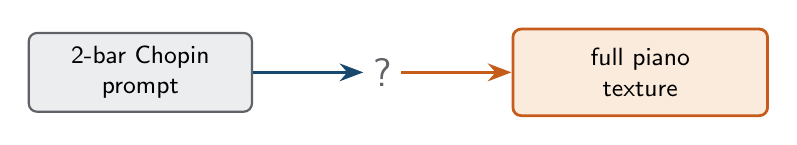
\begin{tikzpicture}[node distance=1.6cm]
    \node[dbox, text width=2.6cm] (p) {2-bar Chopin\\ prompt};
    \node[right=1.4cm of p] (q) {\color{labgray}\Large ?};
    \node[abox, right=1.4cm of q, text width=3.0cm] (o) {full piano\\ texture};
    \draw[flow] (p) -- (q); \draw[flowa] (q) -- (o);
  \end{tikzpicture}
  \note{(Antoine) ``My job is generation. Give the model a melody or a few opening bars, and it should continue or harmonize them the way a real pianist would --- two hands, chords, ornaments, phrasing. That's much harder than generating a single melody line, because piano music is deeply polyphonic and full of notation detail.''}
\end{frame}

% ---- Slide 1.2 — tokenization ----
\begin{frame}{CWT = Compound-Word Transformer}
  \textbf{Key idea:} every musical event = one \alert{compound token} of \textbf{14 parallel heads}, each a different musical dimension.
  \vspace{0.5em}
  \begin{center}\footnotesize
  \begin{tabular}{@{}llll@{}}
    \toprule
    Type & Duration & Pitch(+oct+acc) & Ornament \\
    Articulation & Tie & Slur & Phrase \\
    Voicing & Beam & \textbf{Hand (RH/LH)} & Dynamic \\
    Pedal & Tempo & & \\
    \bottomrule
  \end{tabular}
  \end{center}
  \vspace{0.3em}
  Trained on \textbf{Humdrum **kern} (compact text notation; the KernScores tradition).
  \vspace{0.4em}\par
  \techtag\ \footnotesize 14 categorical heads predicted jointly; total vocab only a \emph{few hundred} tokens vs 20{,}000+ for raw kern $\Rightarrow$ whole pieces fit in a 2{,}048-token window.
  \note{(Antoine) ``The core design is the tokenizer. Instead of one giant vocabulary, I represent each musical event as a compound token --- fourteen parallel heads, each describing one dimension: what type of event, its duration, its pitch, ornament, articulation, which hand plays it, beaming, dynamics, pedal, tempo. The model predicts all fourteen at once. I work in kern, a compact text format for notation with a big ready-made corpus. Remember this fourteen-parallel-heads idea --- it's going to show up again on Harry's side.'' \par [TECH POCKET, optional: each event is 14 categorical heads predicted jointly, and the whole vocabulary across all heads is only a few hundred tokens, versus 20,000-plus for raw kern. That compression is why an entire piece fits in a 2,048-token context window.]}
\end{frame}

% ---- Slide 1.3 — model ----
\begin{frame}{The architecture}
  \begin{columns}[T]
    \begin{column}{0.46\textwidth}
      \begin{itemize}\small
        \item $\sim$\textbf{16.2M-param} Transformer, 10 layers, \alert{RoPE} positions.
        \item \textbf{3-stage cascaded decoding} (models conditional dependencies between attributes).
        \item \textbf{Hand-aware:} declares RH vs LH at every step.
        \item v1 $\to$ v2 (training now) $\to$ v3 (atomic chords).
      \end{itemize}
    \end{column}
    \begin{column}{0.52\textwidth}
      \centering
      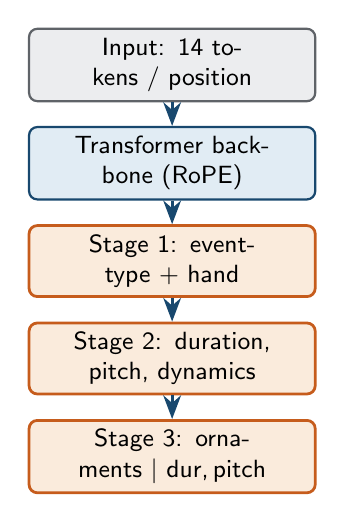
\begin{tikzpicture}[node distance=0.3cm, every node/.style={font=\scriptsize}]
        \node[dbox, text width=3.4cm, minimum height=0.6cm] (in) {Input: 14 tokens / position};
        \node[pbox, below=of in, text width=3.4cm, minimum height=0.7cm] (tr) {Transformer backbone (RoPE)};
        \node[abox, below=of tr, text width=3.4cm, minimum height=0.6cm] (s1) {Stage 1: event-type + hand};
        \node[abox, below=of s1, text width=3.4cm, minimum height=0.6cm] (s2) {Stage 2: duration, pitch, dynamics};
        \node[abox, below=of s2, text width=3.4cm, minimum height=0.6cm] (s3) {Stage 3: ornaments $|$ dur,\,pitch};
        \draw[flow] (in)--(tr); \draw[flow] (tr)--(s1); \draw[flow] (s1)--(s2); \draw[flow] (s2)--(s3);
      \end{tikzpicture}
    \end{column}
  \end{columns}
  \vspace{0.2em}
  \vspace{-0.2em}\par{\techtag\ \scriptsize Stage 3 predicts ornaments \emph{conditioned} on the decided duration \& pitch; embedding is \texttt{concat(14$\times$320)$\to$320}.\par}
  \note{(Antoine) ``The model is a ~16-million-parameter Transformer with rotary position encoding. The clever bit is cascaded decoding in three stages --- it first decides what kind of event this is, then the core attributes like pitch and duration, then the fine ornaments conditioned on those --- because, musically, a trill only makes sense once you know the note's length. And it explicitly tracks which hand is playing. It's gone through three generations: v1 proved the concept, v2 --- training right now --- adds pedaling, tempo, and richer conditioning, and v3 experiments with compressing whole chords into single tokens.'' \par [TECH POCKET, optional: the three stages model the conditional dependencies between attributes explicitly --- ornaments predicted conditioned on the already-decided duration and pitch, not as if the 14 heads were independent. The embedding concatenates all 14 head-vectors and projects them down: concat(14 x 320) to 320.]}
\end{frame}

% ---- Slide 1.4 — data ----
\begin{frame}{$\sim$219{,}000 piano scores}
  \begin{itemize}
    \item \textbf{Sources:} PDMX + ASAP + Chopin first editions + \textbf{KernScores}.
    \item \textbf{Coverage:} $>$99.5\% of pieces fit in a 2{,}048-token window (the model sees whole pieces).
    \item \textbf{Honest status:} v2 is mid-training (epoch 2, loss $\sim$0.076); v1 already produces coherent 6-bar continuations.
  \end{itemize}
  \note{(Antoine) ``It trains on about 219,000 piano scores --- one of the larger symbolic piano corpora assembled for generation --- pulled from public collections and cleaned up. v2 is training as we speak; v1 already generates musically coherent passages from a short prompt. Let me show you.''}
\end{frame}

% ---- DEMO 1 placeholder ----
\begin{frame}[plain]
  \centering\vfill
  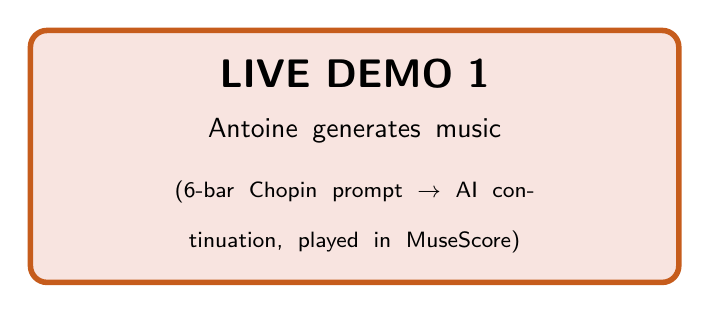
\begin{tikzpicture}
    \node[draw=labaccent, line width=2pt, rounded corners=6pt, fill=boxred,
          text width=8cm, align=center, minimum height=3.2cm, font=\Large\bfseries]
      {LIVE DEMO 1\\[6pt]\normalsize\mdseries Antoine generates music\\[4pt]\footnotesize\mdseries (6-bar Chopin prompt $\to$ AI continuation, played in MuseScore)};
  \end{tikzpicture}
  \vfill
  {\color{labgray}\footnotesize Demo steps + fallback in \texttt{LAB\_PRESENTATION\_SCRIPT.md}}
  \note{DEMO 1 (Antoine). Steps: cd music-cwt/music\_cwt/v2; python gen\_and\_convert.py --prompt-krn ../prompt/nocturne\_op9n1.krn --prompt-measures 6 --temperature 0.8 --top-k 30 --max-tokens 1200. Show the 6-bar prompt, then the AI continuation rendered in MuseScore; hit play. FALLBACK: pre-rendered PDFs/MP3s. SAY: ``These first six bars are the human prompt --- Chopin. Everything after the line is the model. Notice it keeps two real hands, repeats and varies the theme, and stays in key.''}
\end{frame}

% ---- Slide 1.5 — status ----
\begin{frame}{Where Antoine's half stands}
  \begin{itemize}
    \item[\textcolor{labgreen}{\textbf{OK}}] compound tokenizer, v1 generation, kern $\to$ MusicXML $\to$ MuseScore pipeline.
    \item[\textcolor{labaccent}{\textbf{WIP}}] v2 training (pedal/tempo/3-stage), held-out eval set, multi-staff (3+ voices).
    \item[\textcolor{labblue}{\textbf{Next}}] style control (per-composer), longer-range coherence.
  \end{itemize}
  \note{(Antoine) ``So: generation works end-to-end today, v2 is leveling it up, and the open frontiers are longer-range coherence and finer stylistic control. Now --- Harry's half, which is where the surprise lands.''}
\end{frame}

% =====================================================================
\section{Reading music}
% =====================================================================

% ---- Slide 2.1 ----
\begin{frame}{From a performance to a readable score}
  \centering
  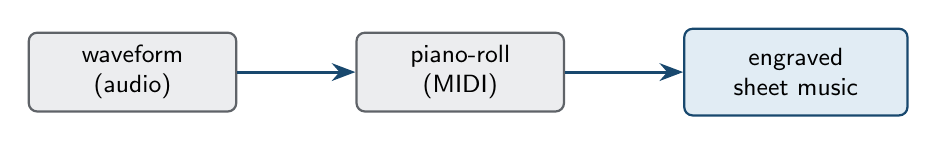
\begin{tikzpicture}[node distance=1.5cm]
    \node[dbox] (a) {waveform\\ (audio)};
    \node[dbox, right=of a] (m) {piano-roll\\ (MIDI)};
    \node[pbox, right=of m] (s) {engraved\\ sheet music};
    \draw[flow] (a)--(m); \draw[flow] (m)--(s);
  \end{tikzpicture}
  \vspace{0.6em}
  \begin{block}{}\centering\footnotesize
    \textit{``What was played''} (messy, expressive timing) $\to$ \textit{``what a musician reads''} (quantized rhythm, beams, voices, hands).
  \end{block}
  \note{(Harry) ``My half is the reverse direction: take sound --- a piano performance --- and write it down as a correct, readable score. The catch is that a performance and a score are very different objects. A performance is expressive, with human rubato and micro-timing. A score is clean and quantized --- bar lines, beams, two staves, voices. Going from one to the other is a hard structured-prediction problem: you have to infer the underlying grid from messy human timing.''}
\end{frame}

% ---- Slide 2.2 — pipeline ----
\begin{frame}{Two blocks}
  \centering
  \resizebox{\textwidth}{!}{%
  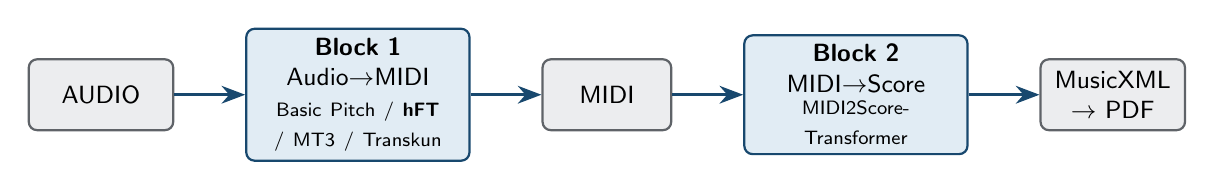
\begin{tikzpicture}[node distance=0.7cm and 0.9cm, every node/.style={font=\scriptsize}]
    \node[dbox, text width=1.6cm, minimum height=0.9cm] (au) {AUDIO};
    \node[pbox, right=of au, text width=2.6cm, minimum height=0.9cm] (b1) {\textbf{Block 1}\\ Audio$\to$MIDI\\ \scriptsize Basic Pitch / \textbf{hFT} / MT3 / Transkun};
    \node[dbox, right=of b1, text width=1.4cm, minimum height=0.9cm] (mi) {MIDI};
    \node[pbox, right=of mi, text width=2.6cm, minimum height=0.9cm] (b2) {\textbf{Block 2}\\ MIDI$\to$Score\\ \scriptsize MIDI2Score-\\Transformer};
    \node[dbox, right=of b2, text width=1.6cm, minimum height=0.9cm] (sc) {MusicXML\\ $\to$ PDF};
    \draw[flow] (au)--(b1);\draw[flow] (b1)--(mi);\draw[flow] (mi)--(b2);\draw[flow] (b2)--(sc);
  \end{tikzpicture}}
  \vspace{0.6em}
  \begin{itemize}\footnotesize
    \item 4 transcribers integrated; \textbf{hFT-Transformer} is best (\textbf{96.7\% onset-F1}).
    \item Block 2 = the Beyer \& Dai model (ISMIR 2024) --- the engine \textbf{Songscription} is built on.
  \end{itemize}
  \techtag\ \footnotesize a path hands the transcriber's float-precision notes \emph{straight} into the score model --- no MIDI-file re-quantization.
  \note{(Harry) ``The system is two blocks. Block 1, audio to MIDI --- which notes were played and when. I integrated four state-of-the-art transcribers; the best is Sony's hFT-Transformer at about 97\% note accuracy. Block 2, MIDI to score --- how do you write those notes down correctly --- uses the MIDI2ScoreTransformer from Beyer and Dai's 2024 paper. And here's a name you'll recognize: that paper's lead author co-founded Songscription, the Shazam for sheet music startup. So Block 2 is literally the engine a commercial product runs on --- which makes it a great, honest yardstick.'' \par [TECH POCKET, optional: we added a path that hands the transcriber's float-precision note events straight into the score model, skipping the MIDI-file round-trip and its re-quantization. Since the whole task is about timing, not throwing timing precision away matters.]}
\end{frame}

% ---- Slide 2.3 — reproduction ----
\begin{frame}{Result \#1: reproduced SOTA --- to within noise}
  \centering
  \begin{tabular}{@{}lcc@{}}
    \toprule
    MUSTER (lower=better) & \textbf{Ours} & Paper (Beyer \& Dai 2024) \\
    \midrule
    \textbf{MeanER} & \textbf{11.18} & 11.30 \\
    PitchER  & 3.19  & 3.11 \\
    MissRate & 7.83  & 7.56 \\
    OnsetER  & 14.50 & 15.55 \\
    OffsetER & 23.73 & 23.84 \\
    \bottomrule
  \end{tabular}
  \vspace{0.6em}
  \begin{center}\footnotesize\color{labgray}
    MUSTER MeanER = the standard score-transcription error rate. All deltas $<$0.12 $\Rightarrow$ \textbf{\color{labblue}validates the whole eval harness.}
  \end{center}
  \techtag\ \footnotesize MUSTER is a C++ aligner over two MusicXMLs (scores \emph{notation}); on Apple Silicon the MPS backend is degenerate $\Rightarrow$ eval runs on CPU.
  \note{(Harry) ``First thing I did was reproduce their result, because you can't improve what you can't measure. On the standard benchmark --- 59 performances, the MUSTER error metric --- we hit 11.18, versus their 11.30. That's within noise. It means our evaluation is trustworthy, and every number after this is measured against a baseline I actually reproduced, not a number from a paper.'' \par [TECH POCKET, optional: MUSTER is a C++ aligner that does a global note-to-note match between two MusicXMLs, so it scores notation, not just note counts. And a real gotcha: on Apple Silicon the MPS backend silently produces degenerate outputs, so the eval has to run on CPU. Finding that is part of why the 11.18 is trustworthy.]}
\end{frame}

% ---- Slide 2.4 — clean piano ----
\begin{frame}{Result \#2: on clean piano, commercial quality}
  \centering
  {\Large Clean piano: end-to-end MeanER \textbf{$\approx$ 2.75}}\par
  \vspace{0.4em}
  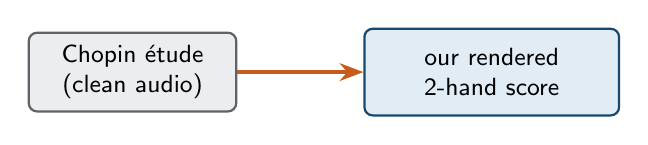
\begin{tikzpicture}[node distance=1.6cm]
    \node[dbox] (a) {Chopin \'etude\\ (clean audio)};
    \node[pbox, right=of a, text width=3.0cm] (s) {our rendered\\ 2-hand score};
    \draw[flowa] (a)--(s);
  \end{tikzpicture}
  \vspace{0.5em}
  \begin{block}{Honest caveat}\footnotesize
    2.75 is the \textbf{easy, in-distribution end} --- \emph{not} a like-for-like win over the product: the score model is the same open checkpoint Songscription runs. The apples-to-apples number is the \textbf{11.18 reproduction}. The hard Romantic repertoire is next.
  \end{block}
  \note{(Harry) ``On clean, in-distribution piano --- Chopin \'etudes from clean recordings --- our full audio-to-score pipeline scores about 2.75. One honest caveat so nobody catches us: that's not a like-for-like win over Songscription. 2.75 is on easy, clean pieces, while the ~11 baseline is the full-test average across all fourteen composers --- and the score model we run is the same open checkpoint Songscription is built on. So the fair claim is: on clean piano, an open pipeline reaches commercial quality, because the score brain is the open part. The apples-to-apples number is the 11.18 reproduction. The interesting science is the hard end --- next slide.''}
\end{frame}

% ---- Slide 2.5 — the ceiling ----
\begin{frame}{Where it breaks: tuplet rhythm}
  \begin{columns}[T]
    \begin{column}{0.5\textwidth}
      \begin{itemize}\small
        \item \alert{Not} the transcriber: \emph{perfect} GT MIDI into Block 2 fails the same way.
        \item \alert{Not} pitch: the notes are right. It's \textbf{where they sit in time} --- triplets/tuplets.
      \end{itemize}
      \vspace{0.4em}
      \textbf{Liszt ``Mazeppa'' ($\sim$49\% tuplets):}\par
      \footnotesize tuplets produced $\approx$ \textbf{half} of GT $\Rightarrow$ wrong meters $\Rightarrow$ \textbf{70\%} too many measures $\Rightarrow$ alignment collapses.
    \end{column}
    \begin{column}{0.5\textwidth}
      \centering
      % 1/24 grid visual
      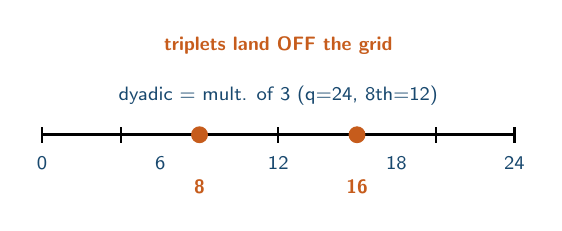
\begin{tikzpicture}[scale=1.0]
        \draw[line width=1pt] (0,0) -- (6,0);
        \foreach \x in {0,1,2,3,4,5,6}{\draw[line width=0.8pt] (\x,-0.1)--(\x,0.1);}
        % dyadic ticks (multiples of 3 on 1/24 grid: 0,6,12,18,24 -> here 0..6 scaled)
        \foreach \x/\lab in {0/0,1.5/6,3/12,4.5/18,6/24}{
          \node[font=\scriptsize, color=labblue, below] at (\x,-0.15) {\lab};}
        \node[font=\scriptsize, color=labblue, above] at (3,0.25) {dyadic = mult. of 3 (q=24, 8th=12)};
        % triplet positions: 8 and 16 -> at 2.0 and 4.0
        \filldraw[labaccent] (2,0) circle (0.10);
        \filldraw[labaccent] (4,0) circle (0.10);
        \node[font=\scriptsize\bfseries, color=labaccent, below] at (2,-0.45) {8};
        \node[font=\scriptsize\bfseries, color=labaccent, below] at (4,-0.45) {16};
        \node[font=\scriptsize\bfseries, color=labaccent, above] at (3,0.9) {triplets land OFF the grid};
      \end{tikzpicture}
      \par\vspace{0.2em}{\footnotesize\color{labgray} grid = 1/24 of a quarter}
    \end{column}
  \end{columns}
  \vspace{0.3em}
  \techtag\ \footnotesize triplets = non-multiple-of-3 buckets (8, 16); individually \emph{rare} $\Rightarrow$ the model learns to never bet on them.
  \note{(Harry) ``When the music gets dense --- late-Romantic, virtuoso --- the pipeline breaks, and I spent a long time finding out exactly where. Two surprises. One: it's not the transcriber. I fed the model perfect ground-truth MIDI and it failed the same way --- so Block 1 is fine. Two: it's not pitch --- the notes are right. The failure is rhythm: specifically triplets and tuplets --- notes that sit between the obvious beats. On a piece that's half tuplets, the model produces only about half the tuplets it should, which forces every note onto a straight grid, which makes it invent the wrong time signature, which inflates the measure count by 70\%, and the whole alignment falls apart. Pitch-perfect, rhythm-broken.'' \par [TECH POCKET, optional: the rhythm grid is one twenty-fourth of a quarter note. Dyadic values land on multiples of three --- a quarter is 24, an eighth is 12 --- and triplets land off them, at 8 and 16. So is-this-a-triplet becomes is-this-onset-on-a-non-multiple-of-three-bucket, and those buckets are individually rare in the data. The model learns to never bet on them.]}
\end{frame}

% ---- Slide 2.6 — the matrix ----
\begin{frame}{Why is tuplet placement so hard? A careful answer}
  \footnotesize
  Diagnostic: the model places \textbf{0\%} of notes at triplet positions on hard pieces (GT $\approx$ 4.8\%).
  \vspace{0.3em}
  \begin{center}
  \begin{tabular}{@{}lcc@{}}
    \toprule
    Lever tried & Triplet placement & MUSTER \\
    \midrule
    Inference cleanup (A2 + pad + per-head) & n/a & \textbf{11.79 $\to$ 11.41} (win) \\
    Corpus reshape ($\gamma$=0.5--1.5)        & 0\% $\to$ \textbf{19.9\%} (over) & regresses \\
    Self-training (pseudo-label MAESTRO)      & 0.9\% & regresses \\
    Loss weighting (tuplet-weight $\times$5)  & 0\% & over-emits \\
    Beat-relative representation (B2)         & 0\% & $\approx$ baseline \\
    Rendered paired (24.73\% triplet targets) & 0\% & undertrained \\
    From scratch (AR undertrained; non-AR matched val) & 0\% & --- \\
    \bottomrule
  \end{tabular}
  \end{center}
  \vspace{0.2em}
  \begin{block}{}\footnotesize
    \textbf{No lever hit the \emph{correct} rate.} Matched the released model's val loss + within $\sim$1 MUSTER pt --- but never its placement. \textbf{Leading explanation: the data} (our corpus is $\sim$1.7\% tuplets). The decisive converged-on-tuplet-rich run is \emph{open} $\Rightarrow$ ``not recovered within our budget,'' \emph{not} ``impossible.''
  \end{block}
  \techtag\ \footnotesize B2 recoding (within-quarter + quarter-index) is lossless \& concentrates 100\% of triplets into shared buckets --- still 0\% learned: representation \emph{necessary, not sufficient}.
  \note{(Harry) ``So I went deep --- and this is the part I'm proudest of, even though it's a negative result, because it's careful. I built a diagnostic: what fraction of notes does the model place at triplet positions? Ground truth is about 5\%. Then I tried to fix it from every angle --- reshaping the data, self-training, a brand-new tuplet-aware representation, cranking the loss, even rebuilding the data engine and training from scratch on 23,000 paired pieces where a quarter of the targets were explicitly triplets. The lever that over-shot hit 20\% --- wrong rate, worse score. Everything else under-shot or collapsed to zero. Nothing hit the correct rate. We matched the released model's validation loss and got within about a point of its benchmark --- but never its correct-rate placement. The leading explanation is the data: our corpus is only about 2\% tuplets. So this isn't a dead end --- it's a data problem, which tells us exactly what to fix, and it's the strongest argument for just using the released model as our engine.'' \par [TECH POCKET, optional: the fix --- B2 --- re-expresses an onset as within-quarter position plus an integer quarter-index, so a triplet becomes the same common bucket in every beat. I proved that recoding is lossless and concentrates 100\% of triplets into shared buckets. And the model still wouldn't learn them without the data --- which is precisely how we know the representation is necessary but not sufficient.]}
\end{frame}

% ---- DEMO 2 placeholder ----
\begin{frame}[plain]
  \centering\vfill
  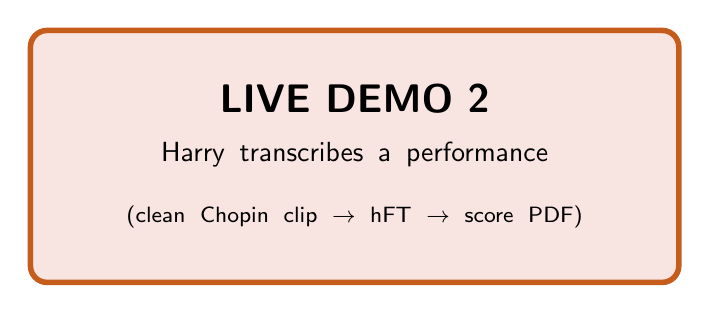
\begin{tikzpicture}
    \node[draw=labaccent, line width=2pt, rounded corners=6pt, fill=boxred,
          text width=8cm, align=center, minimum height=3.2cm, font=\Large\bfseries]
      {LIVE DEMO 2\\[6pt]\normalsize\mdseries Harry transcribes a performance\\[4pt]\footnotesize\mdseries (clean Chopin clip $\to$ hFT $\to$ score PDF)};
  \end{tikzpicture}
  \vfill
  {\color{labgray}\footnotesize Demo steps + fallback PDF in \texttt{LAB\_PRESENTATION\_SCRIPT.md} / \texttt{benchmark/chopin\_op10/transformer/}}
  \note{DEMO 2 (Harry). Steps: python transcribe.py benchmark/chopin\_op10/audio/Op10\_No4\_CsharpMinor.wav -t hft -b transformer. Play ~10s audio, reveal the rendered PDF (two clean staves, correct key, beams). FALLBACK: pre-rendered benchmark/chopin\_op10/transformer/ PDF. SAY: ``That was the raw recording. With one command it becomes this --- two-hand notation, correct key signature, beamed and readable. On clean piano this is essentially product-quality.''}
\end{frame}

% =====================================================================
\section{The convergence}
% =====================================================================

% ---- Slide 3.1 ----
\begin{frame}{Same idea, both halves: multi-head compound tokens}
  \begin{columns}[T]
    \begin{column}{0.5\textwidth}
      \centering\textbf{\color{labblue}Antoine (generation)}\par\smallskip
      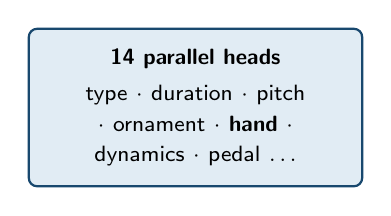
\begin{tikzpicture}\node[pbox, text width=4.0cm, minimum height=2.0cm, fill=boxblue]
        {\footnotesize\textbf{14 parallel heads}\\[2pt]type $\cdot$ duration $\cdot$ pitch $\cdot$ ornament $\cdot$ \textbf{hand} $\cdot$ dynamics $\cdot$ pedal $\dots$};\end{tikzpicture}
    \end{column}
    \begin{column}{0.5\textwidth}
      \centering\textbf{\color{labblue}Harry (transcription)}\par\smallskip
      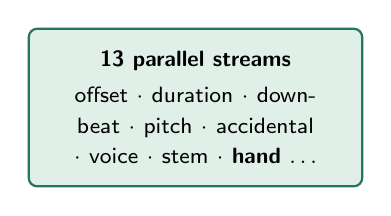
\begin{tikzpicture}\node[pbox, text width=4.0cm, minimum height=2.0cm, fill=boxgreen, draw=labgreen]
        {\footnotesize\textbf{13 parallel streams}\\[2pt]offset $\cdot$ duration $\cdot$ downbeat $\cdot$ pitch $\cdot$ accidental $\cdot$ voice $\cdot$ stem $\cdot$ \textbf{hand} $\dots$};\end{tikzpicture}
    \end{column}
  \end{columns}
  \vspace{0.6em}
  \begin{block}{}\centering
    Two people, two directions, independently chose to represent music as a set of \textbf{parallel attribute streams}. Not a coincidence --- it's the right abstraction for notation.
  \end{block}
  \techtag\ \footnotesize Deeper still: \textbf{both models are RoFormers (RoPE)}. Compound tokens \emph{and} rotary encoding, arrived at independently.
  \note{(Harry) ``Here's the surprise we promised. Antoine and I never coordinated our representations. He encodes each musical event as 14 parallel heads. The transcription model I work on encodes each note as 13 parallel streams --- pitch, duration, voice, stem, hand, and so on. Same idea. Two people, opposite directions, both landed on multi-head compound tokenization because it's the natural way to represent notation: a note isn't one symbol, it's a bundle of attributes.'' \par (Antoine) ``And we both hit the same wall: rhythm and notation fidelity. My generation has to get tuplets, voices, and hands right; Harry's transcription dies on exactly those. The hard problem isn't generation versus transcription --- it's the representation of notation sitting underneath both.'' \par [TECH POCKET, optional: it goes one layer deeper than the tokens. Both models are rotary-position transformers --- Antoine's CWT and the MIDI2ScoreTransformer are both RoFormers, the same positional encoding. So it's compound multi-head tokens and RoPE, chosen independently on both sides --- two people rediscovering the same recipe.]}
\end{frame}

% ---- Slide 3.2 — one system ----
\begin{frame}{One system: the data engine + the generator}
  \centering
  \resizebox{\textwidth}{!}{%
  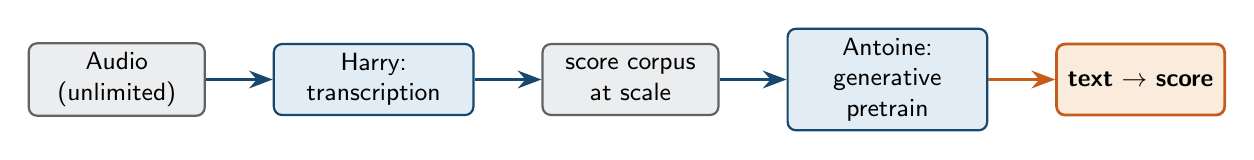
\begin{tikzpicture}[node distance=0.6cm and 0.85cm, every node/.style={font=\scriptsize}]
    \node[dbox, text width=2.0cm, minimum height=0.9cm] (au) {Audio\\ (unlimited)};
    \node[pbox, right=of au, text width=2.3cm, minimum height=0.9cm] (tr) {Harry:\\ transcription};
    \node[dbox, right=of tr, text width=2.0cm, minimum height=0.9cm] (co) {score corpus\\ at scale};
    \node[pbox, right=of co, text width=2.3cm, minimum height=0.9cm] (ge) {Antoine:\\ generative pretrain};
    \node[abox, right=of ge, text width=1.9cm, minimum height=0.9cm] (ts) {\textbf{text $\to$ score}};
    \draw[flow] (au)--(tr);\draw[flow] (tr)--(co);\draw[flow] (co)--(ge);\draw[flowa] (ge)--(ts);
  \end{tikzpicture}}
  \vspace{0.7em}
  \begin{itemize}\footnotesize
    \item Scores are scarce; audio is unlimited. \textbf{Transcription manufactures training data for generation.}
    \item Both stages share \textbf{one notation representation} --- owning it is the lab's real moat.
  \end{itemize}
  \note{(Harry) ``Once you see the shared representation, the two projects click into one system. The bottleneck for any text-to-score generator is paired training data, and scores are scarce. But audio is effectively unlimited. So my transcription pipeline is a data engine: it manufactures large score corpora from audio to pretrain Antoine's generator. That's exactly the moat the commercial players have --- synthetic data at scale. My tuplet finding even tells us which data to trust and which dense-rhythm cases to down-weight so we don't teach Antoine's model bad rhythm.''}
\end{frame}

% ---- Slide 3.3 — division of labor ----
\begin{frame}{Division of labor that actually composes}
  \begin{itemize}
    \item \textbf{Antoine:} the \textbf{generator} (text/melody $\to$ music) + the symbolic-music modeling.
    \item \textbf{Harry:} the \textbf{data engine} (audio $\to$ score at scale) + \textbf{the notation-representation / fidelity} both models depend on.
  \end{itemize}
  \vspace{0.6em}
  \begin{block}{}\centering
    Harry's role isn't ``the transcription guy'' --- it's the \textbf{owner of the shared notation representation}.
  \end{block}
  \note{(Antoine) ``Concretely: I own the generative model and the music modeling. Harry owns the data engine and --- because of the tuplet work --- the notation-fidelity layer that both of our models stand on. That's a division of labor that genuinely composes into the lab's end goal instead of two parallel tracks.''}
\end{frame}

% =====================================================================
\section{The full loop}
% =====================================================================

% ---- Slide 4.1 — the vision end to end ----
\begin{frame}{Text $\to$ Music $\to$ Score --- the whole loop}
  \centering
  \resizebox{\textwidth}{!}{%
  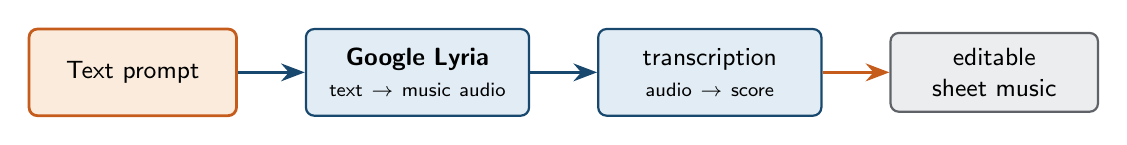
\begin{tikzpicture}[node distance=0.85cm, every node/.style={font=\small}]
    \node[abox, text width=2.4cm] (t) {Text prompt};
    \node[pbox, right=of t, text width=2.6cm] (l) {\textbf{Google Lyria}\\ \scriptsize text $\to$ music audio};
    \node[pbox, right=of l, text width=2.6cm] (tr) {transcription\\ \scriptsize audio $\to$ score};
    \node[dbox, right=of tr, text width=2.4cm] (s) {editable\\ sheet music};
    \draw[flow] (t)--(l);\draw[flow] (l)--(tr);\draw[flowa] (tr)--(s);
  \end{tikzpicture}}
  \vspace{0.7em}
  \begin{center}\footnotesize\color{labgray}\itshape
    A concept demo of the end goal, stitched from today's best pieces --- Lyria for generation, our transcription for notation.
  \end{center}
  \note{(Harry) ``To make the end goal tangible, I built a concept demo of the whole loop using today's best off-the-shelf pieces. You type a description. Google Lyria --- DeepMind's text-to-music model --- turns that text into actual audio. Then the transcription side turns that audio into a score you can read and edit. That's the dream from slide one, working end to end, today.''}
\end{frame}

% ---- DEMO 3 placeholder ----
\begin{frame}[plain]
  \centering\vfill
  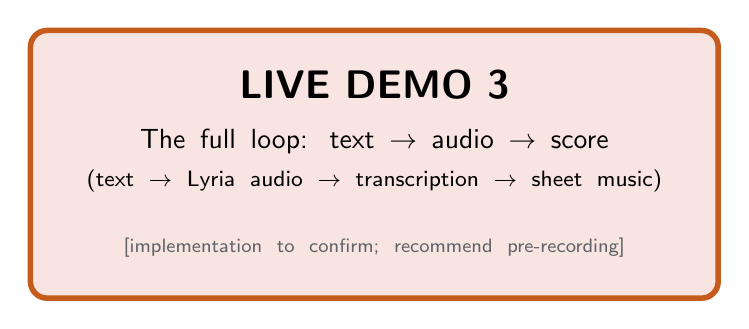
\begin{tikzpicture}
    \node[draw=labaccent, line width=2pt, rounded corners=6pt, fill=boxred,
          text width=8.5cm, align=center, minimum height=3.4cm, font=\Large\bfseries]
      {LIVE DEMO 3\\[6pt]\normalsize\mdseries The full loop: text $\to$ audio $\to$ score\\[4pt]\footnotesize\mdseries (text $\to$ Lyria audio $\to$ transcription $\to$ sheet music)\\[6pt]\scriptsize\mdseries\color{labgray}[implementation to confirm; recommend pre-recording]};
  \end{tikzpicture}
  \vfill
  {\color{labgray}\footnotesize Framing: ``Demo 1 = Antoine's real generator. Demo 2 = my real transcriber. Demo 3 = the vision --- where our two real systems slot in.''}
  \note{DEMO 3 (Harry). Scripted flow: (1) type ``a gentle romantic solo-piano nocturne in A minor''; (2) Lyria generates ~30s audio; (3) feed audio to transcription (Songscription / my pipeline) -> sheet music; (4) show score, play audio. FALLBACK: pre-record the whole screen capture (Lyria can rate-limit). SAY: ``Text in... Lyria gives us audio... and the transcriber writes it down. This is the concept; the part I actually engineered and measured is that transcription step --- which reproduces, and on clean piano matches, the engine Songscription is built on.''}
\end{frame}

% ---- Slide 4.2 — roadmap ----
\begin{frame}{Where this goes (Bayen's direction)}
  \begin{enumerate}
    \item \textbf{Data engine:} transcription manufactures score corpora to pretrain the generator (use the released model as the placement-capable engine; filter dense-tuplet cases).
    \item \textbf{Shared notation representation:} converge our 13/14-head schemes; evaluate a \textbf{rhythm-honest, LLM-friendly format (e.g.\ ABC)} both halves use --- and that makes \emph{text} conditioning natural.
    \item \textbf{Close the loop:} replace Lyria/Songscription in the demo with Antoine's generator + Harry's pipeline $\Rightarrow$ a true \textbf{text $\to$ score} system the lab owns.
  \end{enumerate}
  \note{(Harry) ``Three concrete next steps. One: stand up the data engine --- use transcription to mass-produce training scores for Antoine's generator, with my tuplet findings telling us what to trust. Two: converge our two representations into one shared, rhythm-honest format --- which is also the thing that makes text conditioning natural, the whole point of the lab. Three: close the loop --- swap Lyria and Songscription in that last demo for Antoine's generator and my transcriber, so the text-to-score system is fully ours.''}
\end{frame}

% ---- Slide 4.3 — summary / ask ----
\begin{frame}{Takeaways}
  \begin{itemize}
    \item Two halves --- \textbf{generation (Antoine)} + \textbf{transcription (Harry)} --- both working end-to-end with live demos.
    \item They're \textbf{one system}: same representation idea (compound multi-head tokens + RoPE), same hard problem (notation fidelity), composing into \textbf{text $\to$ score}.
    \item Real results: reproduced SOTA (\textbf{11.18}, within noise), commercial quality on clean piano (\textbf{2.75}), a rigorous characterization of the tuplet ceiling (a \emph{data} problem, not a dead end).
    \item \textbf{The ask:} \rule{4.5cm}{0.4pt} \;{\footnotesize\color{labgray}[compute for the data engine / shared-representation decision / green-light to merge tracks]}
  \end{itemize}
  \note{(BOTH) (Harry) ``To wrap: you saw two real systems --- Antoine's generator and my transcriber --- and a concept demo of the full text-to-score loop.'' (Antoine) ``And the real message is that they're one system: we independently built the same kind of representation and hit the same hard problem, so they belong together.'' (Harry) ``What we'd love from you: [the ask]. Happy to take questions --- and to play more demos.''}
\end{frame}

% ---- Closing ----
\begin{frame}[plain]
  \vfill\centering
  {\color{labblue}\Huge\bfseries Thank you}\par
  \vspace{0.4em}{\color{labaccent}\rule{0.3\textwidth}{1.4pt}}\par
  \vspace{0.8em}{\color{labgray}\large Questions --- and more demos}\par
  \vfill
  \note{Open the floor. Have Appendix backup slides ready (technical deep-dive + anticipated Q\&A).}
\end{frame}

% =====================================================================
\appendix
% =====================================================================
\begin{frame}[plain]
  \centering\vfill
  {\color{labgray}\Large\bfseries BACKUP SLIDES}\par
  \vspace{0.3em}{\footnotesize\color{labgray} anticipated Q\&A + technical deep-dive --- pull up only if asked}
  \vfill
\end{frame}

% ---- Appendix A — anticipated Q&A ----
\begin{frame}{Q\&A: ``Your 2.75 vs 11 --- isn't that cherry-picked?''}
  \footnotesize
  Yes, deliberately, and we flag it: 2.75 is the clean in-distribution end; the 11 is the full-test average. The honest, apples-to-apples number is the \textbf{11.18 reproduction}. 2.75 shows the \emph{ceiling} of what's possible on the music it's designed for; the tuplet finding shows the \emph{floor} on hard music.
\end{frame}

\begin{frame}{Q\&A: ``Did you just not train long enough?''}
  \footnotesize
  Honest answer: partly --- our capstone from-scratch run was \textbf{undertrained}, so we can't claim impossibility. What we \emph{can} say is sharper: a model that matched the released \emph{validation loss} still showed zero correct-rate placement, and pushing it with data, representation, and loss never hit the correct rate. Leading explanation: the \textbf{data} (corpus $\sim$1.7\% tuplets). So it's ``not recovered within our compute/data budget; the data is the binding constraint'' --- pointing to a concrete fix (tuplet-rich corpus, trained to convergence). One cheap step not yet done: email the paper's author.
\end{frame}

\begin{frame}{Q\&A: novelty vs.\ off-the-shelf; data engine real?}
  \footnotesize
  \textbf{Novel:} (1) the rigorous, controlled characterization of the tuplet-placement ceiling (unpublished); (2) the data-engine framing (turn unlimited audio into scarce score data); (3) the convergence insight (generation + transcription share one representation).\par\medskip
  \textbf{Data engine real?} The pieces are real --- a transcription pipeline that reproduces SOTA + a render/pairing pipeline that already built a 23{,}000-piece paired corpus in minutes. Aspirational: scaling it and wiring it into pretraining --- that's the ask.
\end{frame}

% ---- Appendix D — technical backup ----
\begin{frame}{D1 --- The two tokenizers, side by side}
  \scriptsize
  \begin{columns}[T]
    \begin{column}{0.5\textwidth}
      \textbf{Antoine --- CWT, 14 heads}\par
      Type, Duration, Pitch(+oct+acc), Ornament, Articulation, Tie, Slur, Phrase, Voicing, Beam, \textbf{Hand}, Dynamic, Pedal, Tempo.\par\smallskip
      Vocab $\approx$ few hundred; \texttt{concat(14$\times$320)$\to$320}; \textbf{RoPE}; 3-stage decode; $\sim$16.2M params; autoregressive.
    \end{column}
    \begin{column}{0.5\textwidth}
      \textbf{Harry --- MIDI2ScoreTransformer, 13 streams + pad}\par
      offset, downbeat, duration, pitch, accidental, keysignature, velocity, grace, trill, staccato, voice, stem, \textbf{hand}, + \texttt{pad} gate.\par\smallskip
      \textbf{RoFormer} enc-4/dec-4, hidden 512, 8 heads, $\sim$32.6M params; non-autoregressive (mask-predict).
    \end{column}
  \end{columns}
  \vspace{0.5em}
  \begin{center}\color{labblue}\textbf{Shared, unplanned: compound multi-head tokens + RoPE.}\end{center}
\end{frame}

\begin{frame}{D2 --- MUSTER, in detail}
  \footnotesize
  Python wrapper around a \textbf{C++ aligner} over two MusicXMLs. Six error rates --- PitchER, MissRate, ExtraRate, OnsetER, OffsetER $\to$ \textbf{MeanER} (their mean). Plus engraving sub-metrics (note spelling, voice assignment, stem direction, staff assignment) + voice precision/recall/F1. \textbf{Aborts on 3-staff scores} (limits OOD eval). Our 11.18 matched the paper on \emph{all five} sub-metrics within 0.12.
\end{frame}

\begin{frame}{D3 --- The 1/24 grid + the placement diagnostic}
  \footnotesize
  Grid = \textbf{1/24 of a quarter}. Dyadic = multiples of 3 (quarter 24, eighth 12, 16th 6); triplet/sextuplet = off-multiples (8, 16, 4, 20). \texttt{diag\_offset\_phase.py} measures the fraction of onsets at triplet phases: \textbf{GT $\approx$ 4.78\%, our models 0\%}.\par\smallskip
  \textbf{B2} = within-quarter offset + integer \texttt{quarter\_idx}. Verified: lossless round-trip, 100\% triplet concentration into shared buckets, non-B2 byte-identical. Conclusion: representation \textbf{necessary, not sufficient}.
\end{frame}

\begin{frame}{D4 --- The exhaustive placement matrix + data engine}
  \footnotesize
  Inference cleanup $\to$ 11.79$\to$\textbf{11.41} (only robust gain); global logit-shift $\to$ over-emits; corpus reshape $\to$ \textbf{19.9\%} (over-shoots, regresses); self-training $\to$ 0.9\%; tuplet-weight $\times$5 $\to$ 0\%; B2 $\to$ 0\%; paired distillation (2.87\% targets) $\to$ 0\%; rendered paired (\textbf{24.73\%} targets) $\to$ 0\% (undertrained); from-scratch AR (val 1.3, undertrained) + non-AR (matched val 0.51) $\to$ 0\%.\par\smallskip
  \textbf{Data engine:} 23{,}780 PDMX scores rendered $\to$ valid per-beat-aligned paired data in $\sim$11 min; tuplet-rich subset 24.73\% placement.
\end{frame}

\begin{frame}{D5 --- Eval-harness rigor (why the numbers are real)}
  \footnotesize
  \begin{itemize}
    \item \textbf{MPS$\to$CPU:} Apple-MPS produced degenerate pad logits $\Rightarrow$ eval forced to CPU.
    \item \textbf{val $\neq$ MUSTER:} re-rank checkpoints by \emph{true} MUSTER, not loss.
    \item \textbf{Leakage audit:} 12/17 eval pieces found in PDMX via \emph{content fingerprints} (transposition-invariant interval n-grams, not titles) $\Rightarrow$ content-dedup tool + blocklist for future training.
    \item \textbf{Pad-threshold bug:} released \texttt{generate()} hard-argmaxed \texttt{pad} to binary (any threshold a no-op) --- we fixed it (continuous keep-probability + un-zeroed raw streams).
  \end{itemize}
\end{frame}

\end{document}
